\section{System Performance Analysis}
\label{sec:system_performance_analysis}

\newcommand{\TMAMotionSettings}{\href{https://rubinobs.atlassian.net/wiki/spaces/LSSTCOM/pages/53741249/TMA+Motion+Settings}{TMA Motion Settings}}

Topics to convert into text

\begin{itemize}
    - M1M3 and M2 glass installed on the Simonyi Survey Telescope.
    - Since then, we have been operating the telescope with limited velocity,
    acceleration, and jerk limits following the performances defined in \TMAMotionSettings.
    - For each configuration, defined in terms of a percentage of the maximum
    velocity, acceleration, and jerk, we ran multiple gateway tests.
    - The gateway tests are described in the subsection \ref{subsec:gateway_tests} below.
\end{itemize}

\subsection{Gateway Tests}

The three gateway tests defined below are required for each increase in the
velocity, acceleration, and jerk limits. They are associated with glass and
telescope safety. So far, we have been able to run the telescope up to 10\%
its maximum velocity, acceleration, and jerk limits. For simplicity, we will
show only the last results.

\subsubsection{Long and short slews at different elevations}
\label{subsubsec:long_and_short_slews}

These tests ensure that the force balance systems on M1M3 and on M2 can protect
the mirrors on different telescope positions and while slewing. As we increase
velocity, acceleration, and jerk limits, both mirrors suffer higher inertial
forces and the force actuators must counteract them.

For M1M3, the criteria is to keep the measured forces on the hardpoint actuators
below the operational limit (15\% the breakaway limit). For M2, the criteria is
??????? (check with Holger, Gabriele, and Pablo). % TODO - check with

Test cases associated:
\begin{itemize}
    - \href{https://rubinobs.atlassian.net/projects/BLOCK?selectedItem=com.atlassian.plugins.atlassian-connect-plugin:com.kanoah.test-manager__main-project-page#!/v2/testCase/BLOCK-T227}{BLOCK-T227 Dynamic Tests at El = 34º - short and long slews}
    - \href{https://rubinobs.atlassian.net/projects/BLOCK?selectedItem=com.atlassian.plugins.atlassian-connect-plugin:com.kanoah.test-manager__main-project-page#!/v2/testCase/BLOCK-T293}{BLOCK-T293 Dynamic Tests at El = 70º - short and long slews}
    - \href{https://rubinobs.atlassian.net/projects/BLOCK?selectedItem=com.atlassian.plugins.atlassian-connect-plugin:com.kanoah.test-manager__main-project-page#!/v2/testCase/BLOCK-T294}{BLOCK-T294 Dynamic Tests at El = 70º - short and long slews}
    - \href{https://rubinobs.atlassian.net/projects/LVV?selectedItem=com.atlassian.plugins.atlassian-connect-plugin:com.kanoah.test-manager__main-project-page#!/v2/testCase/LVV-T2813}{LVV-T2813 M1M3 Dynamic Test, increasing speed, increasing acceleration}
    - \href{https://rubinobs.atlassian.net/projects/LVV?selectedItem=com.atlassian.plugins.atlassian-connect-plugin:com.kanoah.test-manager__main-project-page#!/v2/testCase/LVV-T2944}{LVV-T2944 M2 Dynamic Test, increasing speed, acceleration, jerk}
\end{itemize}

Detailed analysis (both TNs are still under development):
\begin{itemize}
    - \href{https://sitcomtn-092.lsst.io/}{SITCOM-TN092 M1M3 Force Balance System - Inertia Compensation}
    - \href{https://sitcomtn-147.lsst.io/}{SITCOM-TN147 M2 Response to short and long slews}
\end{itemize}

\begin{figure}
    \centering
    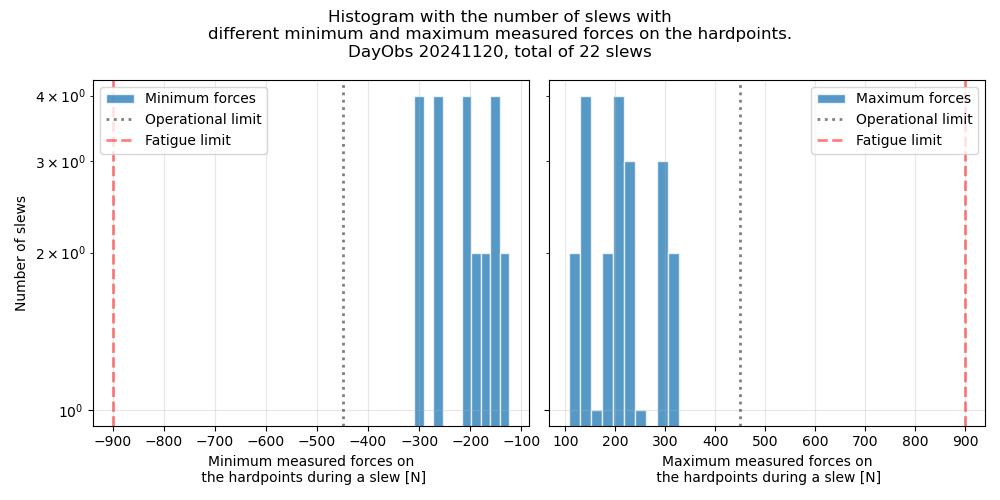
\includegraphics[width=0.8\textwidth]{spa/M1M3_short_long_slews_10_histogram.png}
    \caption{Number of slews with minimum/maximum measured forces on the M1M3 hardpoint actuators.}
    \label{fig:m1m3_short_long_slews}
    \end{figure}

\begin{figure}
    \centering
    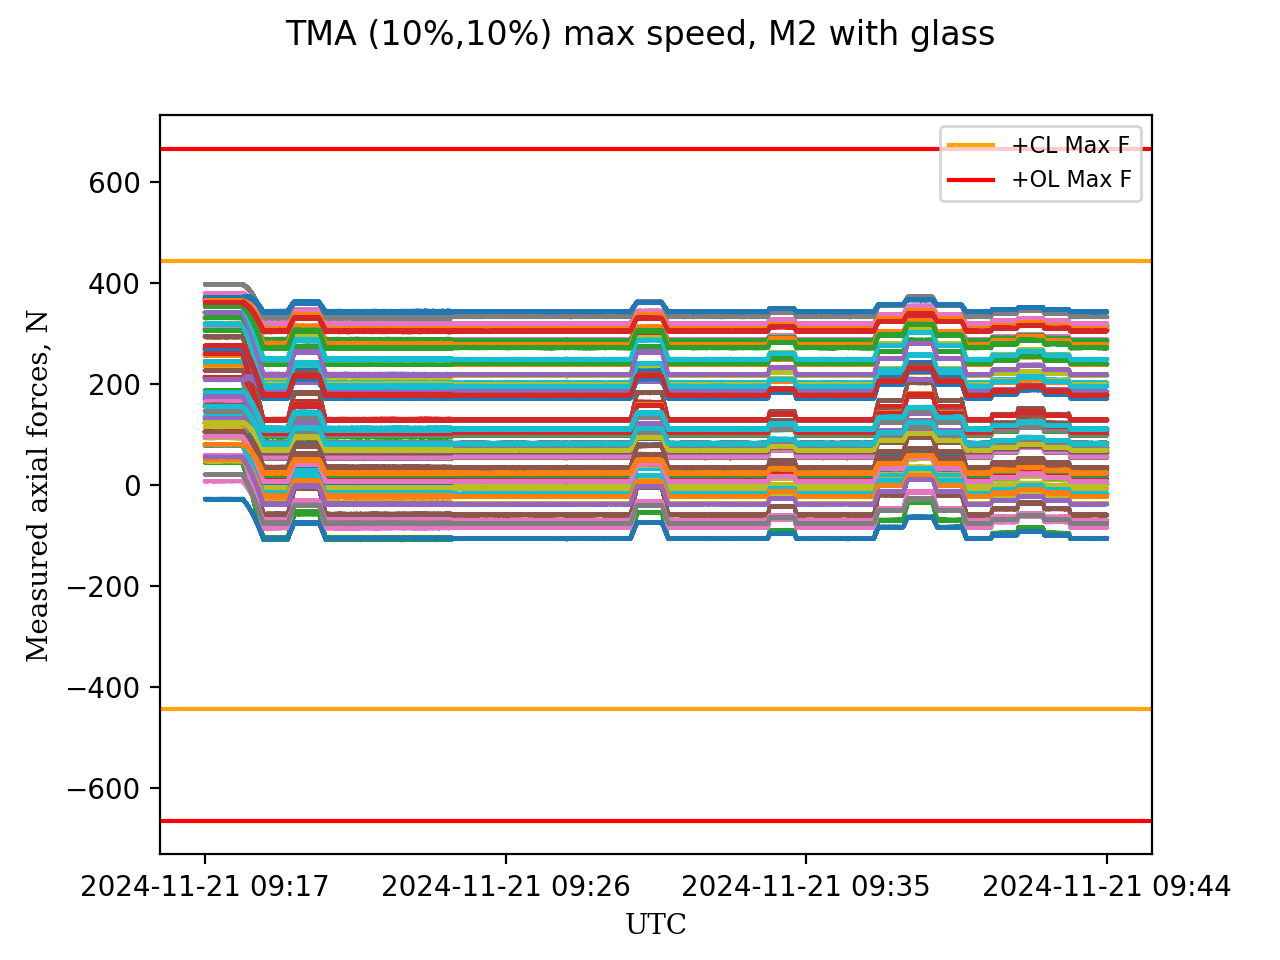
\includegraphics[width=0.8\textwidth]{spa/M2_short_long_slews_axial_measured_force_10.png}
    \caption{Measured axial force on the M2 force actuators during short and long slews.}
    \label{fig:m2_short_long_slews_axial}
    \end{figure}

\begin{figure}
    \centering
    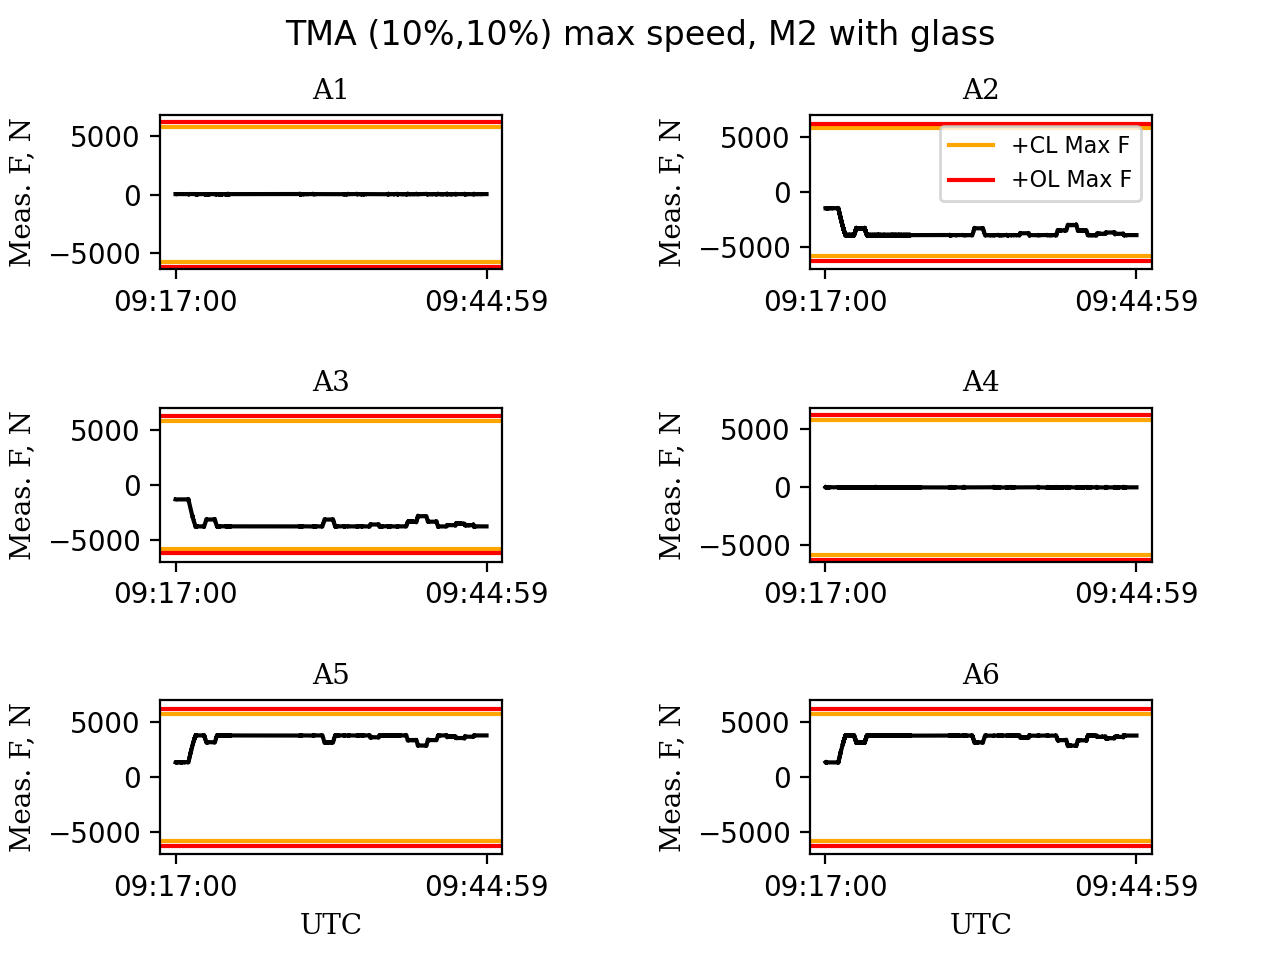
\includegraphics[width=0.8\textwidth]{spa/M2_short_long_slews_Tangent_measured_forces_TMA_10.png}
    \caption{Measured tangent force on the M2 force actuators during short and long slews.}
    \label{fig:m2_short_long_slews_tangent}
    \end{figure}

\begin{figure}
    \centering
    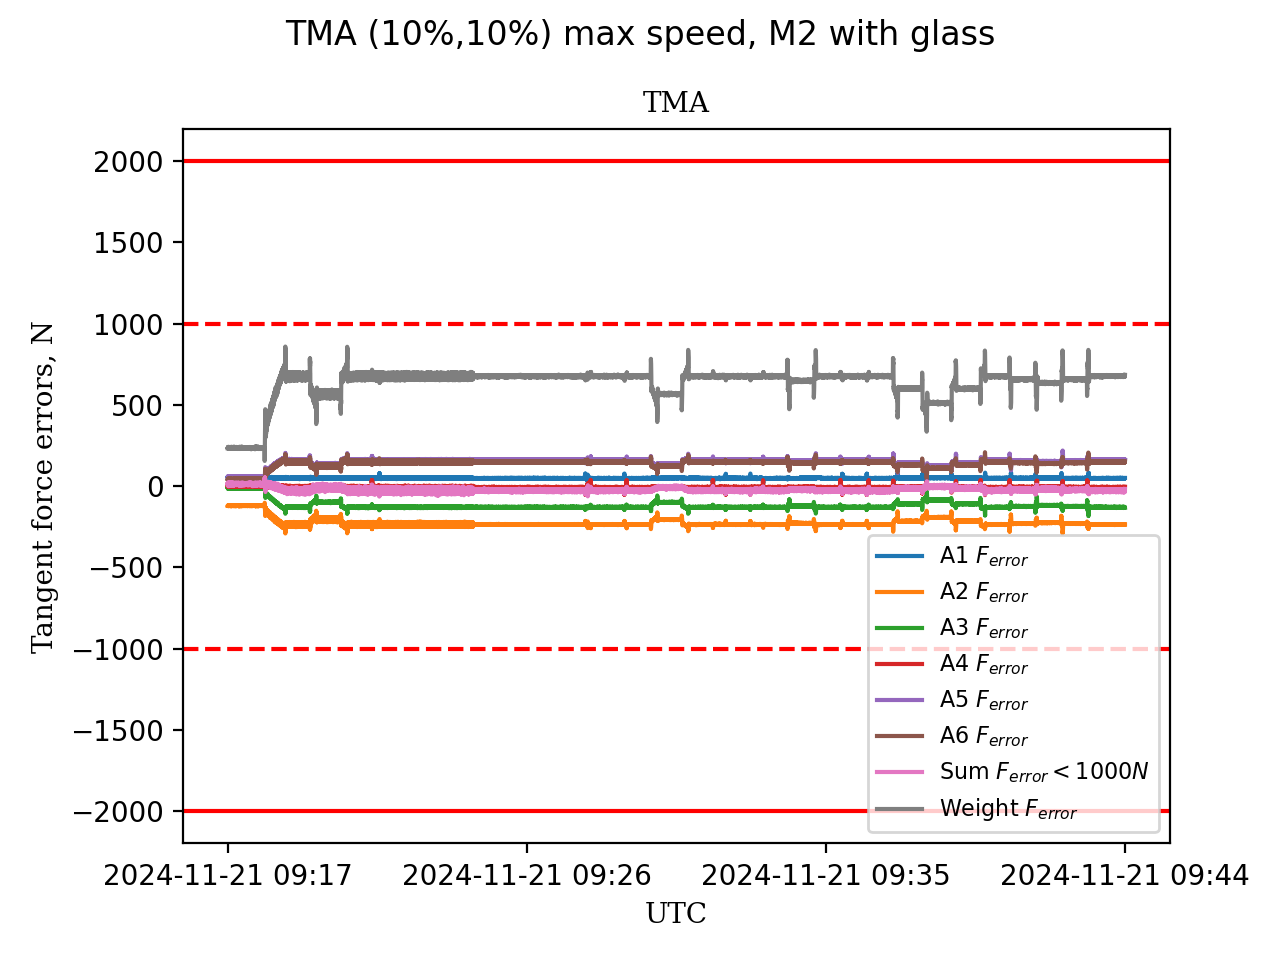
\includegraphics[width=0.8\textwidth]{spa/M2_short_long_slews_tangent_force_errors_10.png}
    \caption{Measured tangent force errors on the M2 force actuators during short and long slews.}
    \label{fig:m2_short_long_slews_tangent_errors}
    \end{figure}

\subsubsection{M2 close-loop breakout tests}
\label{subsubsec:m2_close_loop_breakout_tests}

\subsubsection{TMA azimuth and elevation brake tests}
\label{subsubsec:tma_azimuth_and_elevation_brake_tests}

